\section{Literature Review}

\label{sec:review}

\subsection{Introduction}

The majority of mobile platforms or unmanned vehicles in use today are non-holonomic.
They only have one or two degrees of freedom that are independent.
As a result, its maneuverability is limited, and it frequently requires a large amount of space to control functions such as turning and parking.
This can be seen when a car wants to turn 180\degree.
By increasing a vehicle's degrees of freedom we are improving its maneuverability.
It can follow many complex trajectories that conventional nonholonomic vehicles find difficult or impossible.
Holonomic refers to the relationship between controllable and total degrees of freedom of a robot.
A holonomic platform is any mobile platform with three independent degrees of freedom in a plane.
If the controllable degree of freedom is equal to the total degrees of freedom, then the robot is said to be holonomic.
Independent degrees of freedom indicate that it can change its orientation or position without affecting other motions, as opposed to car-type vehicles, which must turn or change their orientation when moving.
A robot built on castor wheels or Omni-wheels is a good example of a holonomic drive as it can freely move in any direction and the controllable degrees of freedom is equal to total degrees of freedom. 


\subsubsection{Mobile platforms}

Over the last three decades, researchers have been working on omnidirectional wheeled mobile robots.
There are also legged mobile robots which achieve both holonomic and omnidirectional motion.
Legged mobile platforms have the advantage of highly adapted to uneven terrain, low soil interaction and the ability to perform tasks in congested and narrow environments.
Nevertheless, their slow mobility, low payload weigh to mechanism weight ratio, complex design and control makes them difficult to find\cite{seeni_2008}.

\subsubsection{Castor Wheel}

A castor or caster wheel is a relatively free-rolling ,not powered, small undriven wheel.
They are designed to be attached to the bottom of a larger object, to enable easy movement across a floor or other hard surface.
Castor wheels are manufactured in either a single wheel, double wheel, or compound wheel configuration.
\par
Most castors are used simply to make a heavy or cumbersome piece of furniture or machinery - the vehicle - easier to move.
Affixing small, unobtrusive wheels to the bottom of any large or bulky item is a great way to make it more mobile in certain scenarios.
In most cases, they are attached to the underside of the vehicle via a fixed top plate, from which the wheel assembly hangs.
\par
When choosing the type of casters to use in an application, weight considerations need to be considered depending on the load the casters will be required to move.
To achieve this, we need to consider the weight of the item being supported as shown by equation \ref{eq:1}.

\begin{equation}
\label{eq:1}
total\:load\:capacity = individual\:weight\:rating * number\:of\:wheels
\end{equation}

The total load-bearing capacity of your castors should always be at least 30\% higher than the total weight of the item when fully loaded, to give a sufficient safety margin.
Another consideration to take into account is the type of surface the castors will be moving on.
These surfaces are either flat and smooth that can accommodate small wheels or rougher surfaces that require wheels with larger diameters.
There are several types of castors each suited to a different application.
The most common casters are as shown by figure \ref{fig:polyurethanecastorwheels}, figure \ref{fig:synthetictreadwheels} and figure \ref{fig:ferrouscasterwheels}

\begin{figure}[htbp]
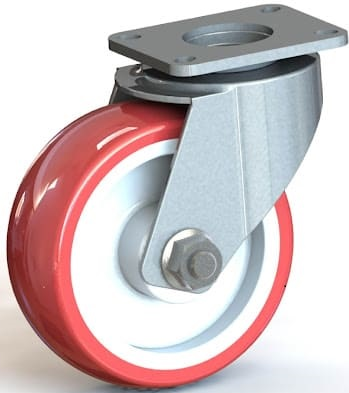
\includegraphics[scale=0.3]{Figures/polyurethane-caster-wheel.png}
\centering
\caption[Polyurethane Castor Wheels] {Polyurethane Castor Wheels	 \cite{noauthor_caster_nodate}.}
\label{fig:polyurethanecastorwheels}
\end{figure}

\begin{figure}[htbp]
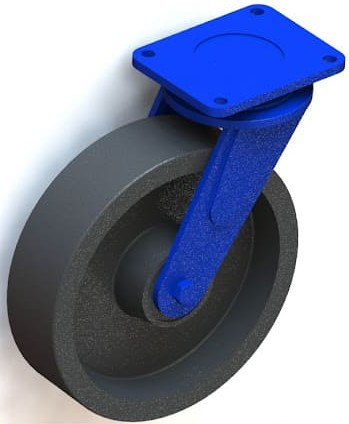
\includegraphics[scale=0.3]{Figures/synthetic-tread-wheels.jpg}
\centering
\caption[Synthetic Tread Wheels] {Synthetic Tread Wheels	 \cite{noauthor_caster_nodate}.}
\label{fig:synthetictreadwheels}
\end{figure}

\begin{figure}[htbp]
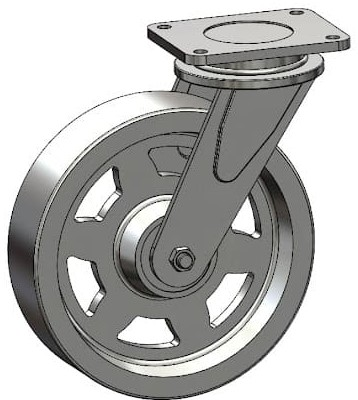
\includegraphics[scale=0.3]{Figures/ferrous-caster-wheel.jpg}
\centering
\caption[Ferrous Caster Wheels] {Ferrous Caster Wheels	 \cite{noauthor_caster_nodate}.}
\label{fig:ferrouscasterwheels}
\end{figure}

Ferrous wheels, Figure \ref{fig:ferrouscasterwheels} provide the highest load capacity, impact resistance, temperature range, and rollability of any caster wheel available due to their solid structure, making them excellent for harsh situations such as warehouses and manufacturing factories where a floor protection is not a priority.
Polyurethane tread wheels, Figure \ref{fig:polyurethanecastorwheels} provide good floor protection and have a 3,000-pound capacity and strong impact resistance \cite{noauthor_caster_nodate}.
Synthetic wheels Figure \ref{fig:synthetictreadwheels}, have a harder tread with lower rolling resistance and higher impact strength and reliability.
While most synthetic wheels are ideal for high-impact and harsh situations, they are louder than softer materials and are less forgiving when colliding with debris. 

\subsection{Existing Technologies}

\subsubsection{Wheel design}

For wheeled mobile robots, we have \cite{muir_kinematic_1987}: conventional wheels, omnidirectional wheels, and ball wheels.
The conventional wheels are the ones we see on cars and trolleys every day.
An omnidirectional wheel is a disk-shaped wheel with numerous conventional wheels mounted on its periphery.
A ball wheel \cite{ostrovskaya_dynamics_2000}, \cite{west_design_1995} is shaped like a ball but its implementation is difficult because including an axle in the design sacrifices usable workspace.
It is also difficult to provide power transmission to the wheel.
For large and heavy outdoor robots, four-wheel or car-like driving mechanisms have traditionally been used.
Because the non-holonomic constraints on their wheel mechanisms prevent sideways movements, these vehicles are quite restricted in their motion \cite{laumond_feasible_1986}\cite{pin_autonomous_1990}\cite{noauthor_navigation_nodate}, especially when operating in tight environments.
Improved motion capabilities have been investigated in a number of research centers and demonstrated on laboratory robots.
These motion capability enhancements are typically derived from the use of two independent driving wheels supplemented by casters.
This allows the platform to rotate around any point but does not allow for sideways motion.
Another motion can be achieved using two steerable and independently driving wheels \cite{pin_autonomous_1989}, or three steerable and coordinated driving wheels \cite{pin_autonomous_1989}.
These two implementations allow for both platform rotation and sideways motion through coordinated steering of the wheels.
However, in these latter systems, the controls for translational and rotational motions are not fully decoupled or independent, as very strict compatibility conditions exist between the steering and driving velocities of the wheels \cite{alexander_kinematics_1989}.
To achieve the full three degrees of freedom of planar rigid body motion, these platforms must be controlled as strongly constrained systems.
Furthermore, steering necessitates the rotation of the wheels around a vertical axis, which, in the case of heavy payloads or vehicles with wide tires, may result in significant wheel sliding and friction.
The traditional wheel is probably the simplest and most durable of the designs. However, not all conventional wheels can provide omnidirectional motion \cite{muir_kinematic_1987} \cite{alexander_kinematics_1989} \cite{ostrovskaya_nonholonomic_1998}. It is widely accepted that caster design provides full mobility \cite{d39_structural_1996}.
Mecanum wheels also achieve holonomic and omnidirectional motion by having a series of rollers attached to their circumference \cite{diegel_improved_nodate}.
These rollers have an axis of rotation at 45\degree to the plane of the wheel.
The angled peripheral rollers translate a portion of the force in the rotational direction of the wheel \cite{diegel_improved_nodate}.
Each mecanum wheel in a drive system has independent actuation and the resulting combination of forces to move these wheels produces a total force vector that allows the platform to move freely in any direction.
Different variations of mecanum wheels depend on the number of rollers attached to individual wheels, as shown in figure \ref{fig:differentvariationsofmecanumwheels}.


\begin{figure}[htbp]
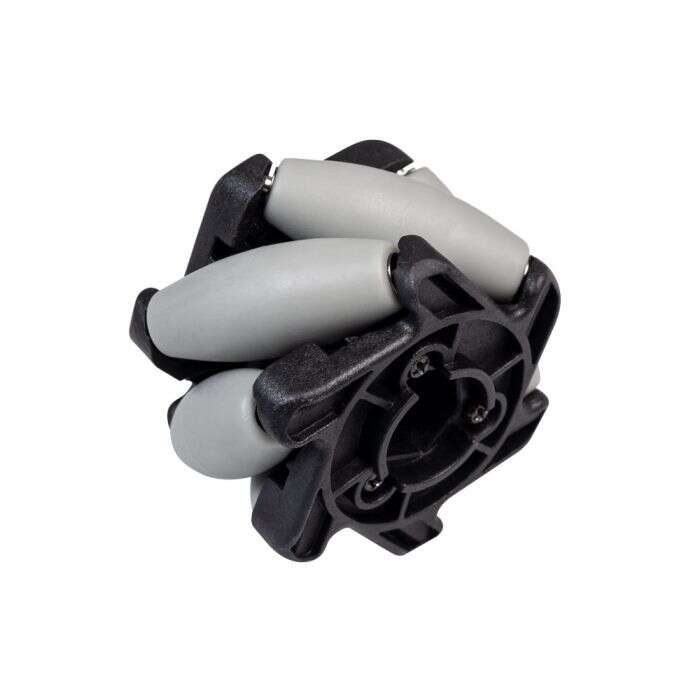
\includegraphics[scale=0.4]{Figures/mecanum1.jpg} 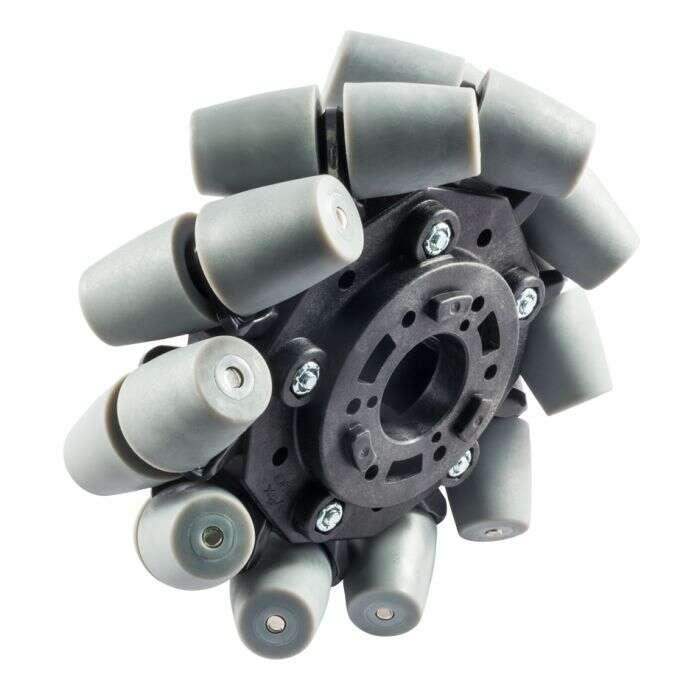
\includegraphics[scale=0.3]{Figures/mecanum2.jpg} 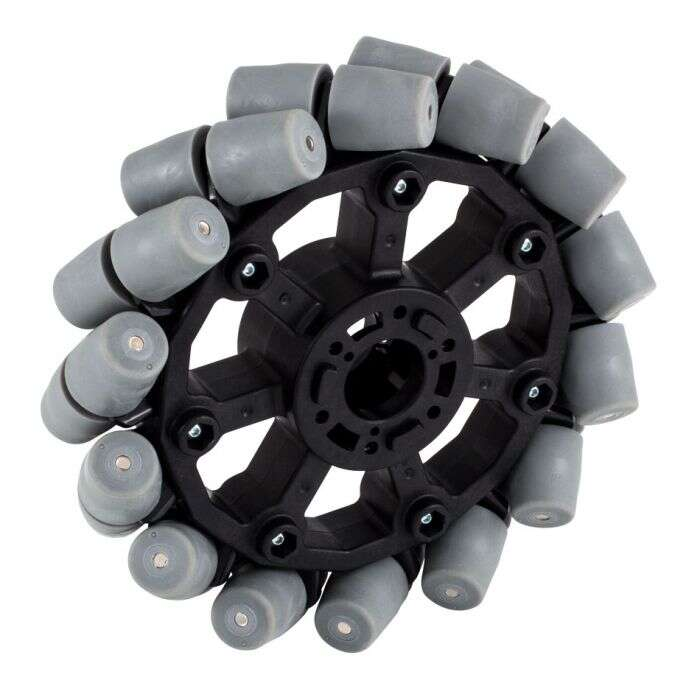
\includegraphics[scale=0.3]{Figures/mecanum3.jpg}\centering
\caption[Different variations of mecanum wheels] {Different variations of mecanum wheels \cite{diegel_improved_nodate}.}
\label{fig:differentvariationsofmecanumwheels}
\end{figure}

In the development of mecanum and other omnidirectional wheels \cite{kim_design_2001}\cite{paromtchik_practical_1994}, undesirable vibrations are frequently present in the motion due to a large number of small rollers on the wheel's periphery.

\subsubsection{Omnidirectional and holonomic motion}

A lot of design work on omnidirectional vehicles has been conducted over the years.
The earliest omnidirectional mobile vehicle to be proposed was based on introducing a methodology for the kinematic modelling of an omnidirectional wheeled mobile robot equipped with four omnidirectional wheels which were based on passive rollers arranged
in an overlapping way \cite{javier_moreno_design_2016}.
These wheels were positioned in pairs on the same axle but with opposite orientations.
Another proposal by Wada and Mori \cite{wada_holonomic_1996} presented a new type of holonomic mobile robot which was equipped with steerable and coordinated driving wheels using conventional tires to provide an omnidirectional capability by actuating the wheels axis and a steering axis independently.
In another paper by Javier Moreno, Eduard Clotet, and others design \cite{javier_moreno_design_2016} validate a three-wheel holonomic motion system for an assistant personal robot.
The paper analyzes the kinematics of the motion system and validates the estimation of the trajectory by comparing the displacement estimated with the internal odometry of the motors and the displacement estimated with a \ac{SLAM} procedure based on \ac{LIDAR} information . 

\subsection{Gap Analysis}

Huge leaps have been made in the development of mobile vehicles or robots with holonomic and omnidirectional motion.
Mecanum wheels have taken center stage, and the use of rollers attached to a conventional wheel has found great applications in small-scale robots and mobile platforms.
However, these wheels cannot be applied to certain applications that involve heavy payloads or rough terrains.
Such applications are moving objects in warehouses or factory floors.
Castors are predominantly used in these areas, but it involves manual control.
This process can be automated by modifying the castors by adding motors for directional control and adding the concept of remote control.
This, however, has not been adopted which necessitates this research.


% \begin{equation}
% \dot{x}=Ax+Bu+B_dw
% \end{equation}
% %
%  Refering a chapter in the main text. For instance Chapter~\ref{sec:review} 
% %
% \begin{eqnarray} \nonumber
% E = 210000\Unit{\mathrm{\frac{N}{mm^2}}}
% \end{eqnarray}
% %

% %
% \begin{eqnarray}
% K_\varphi & = & 3.64\;\mr{\frac{V}{rad}}\quad\mbox{and}\\
% K_x & = & 28.32 \;\mr{\frac{V}{m}}.
% \end{eqnarray}
% %

